\chapter{Asking a Tech Millionaire How to Start \& Scale a Tech Company}

This chapter reads a School of Hard Knocks interview, curated by LazyingArt LLC, as a compact lecture on startup method. We begin in a deliberately broad register, with teaser questions, public rejections, and quick fragments of business advice. Only afterward does the lecture settle into its real line of argument: how a founder validates an idea, decides whether it deserves more capital, resists perfectionism, raises money from traction rather than fantasy, and thinks about scale, exit, and a second company.

\begin{remark}
No validated board screenshots survived for this lecture. The formulas and diagrams below are therefore transcript-derived reconstructions of the interview's operational logic, not transcriptions of visible board notation.
\end{remark}

\section{Prologue: Pressure Before Procedure}

The lecture opens on the way to meet John Abraham, and the opening is not yet explanatory. It is promissory. We are told what kind of case we are about to hear: a founder who has already launched, exited, and started again. The first questions are the ones the whole chapter will keep returning to: how do we start, how do we scale, how do we raise capital, and how does a business become sellable?

The early montage widens the field before it narrows it. We hear from a retired technology salesperson who attributes very large earnings to stock options and therefore to ownership, not merely salary. We hear a government worker turned consultant, then a speaker who insists that success in business demands both assertiveness and professionalism, and then another who recommends a niche, hard work, and the discipline to cut a bad direction quickly. These fragments matter because they preload the lecture's recurring motifs: ownership rather than pure labor, relationships rather than transaction, and operating judgment rather than glamour.

Another theme is introduced through embarrassment rather than doctrine. The hosts are ignored, rejected, and sometimes cursed at. The narration then turns this into a rule of the world: rejection belongs to the process. Before we ever arrive at John Abraham's more systematic advice, the lecture has already placed the entrepreneur in public, where refusal is ordinary and progress requires persistence.

\section{From Street Advice to a Founder With a Timeline}

The lecture then resets itself. The hosts explain that they had earlier overheard John Abraham talking business at a restaurant, discovered that he had already sold one company and was building another, and returned to record a more sustained conversation. This is a structural pivot. We move from ambient business culture to a founder case study that can bear a more continuous argument.

John's authority is established through chronology. He bartended in college, watched people from Dell, Applied Materials, and Intel come through, wanted entry into the technology world, and pushed until he got a chance in tech sales. Only then does the lecture place the key dates:
\begin{equation}
t_{\mathrm{launch}} = 2014,\qquad
t_{\mathrm{exit}} = 2018,\qquad
\Delta t_{\mathrm{launch\to exit}} = 4\ \text{years}.
\end{equation}
This is not a deep theorem, but it is an important anchor. The advice that follows is not abstract startup folklore. It comes from a founder who took one application from launch to exit in four years and is now building again.

The second company, Haymaker, is introduced in plain terms: a marketplace, somewhat like Airbnb in form, but aimed at temporary office and meeting space. The lecture does not linger yet. It names the object, then postpones the worked example until the end, when we will be in a better position to understand why this particular kind of marketplace matters.

\section{Customer Discovery Before Product}

\subsection{Question \& Answer}

The first real operational question is posed directly: how do we turn an idea into action? John's answer is immediate and corrective. We do not begin by building. We begin by learning whether there is anything here to build.

\begin{definition}
For compactness, we introduce a small notation bank:
\[
D = \text{customer-discovery interviews},\qquad
P = \text{pain points},
\]
\[
V = \text{business-value test},\qquad
\Pi = \text{pilot commitment},
\]
\[
\mathrm{TAM} = \text{total addressable market},\qquad
\mathrm{MVP} = \text{minimum viable product}.
\]
These symbols abbreviate a spoken sequence from the interview.
\end{definition}

The lecture's most important early ordering claim may be written as
\begin{equation}
D \rightarrow P \rightarrow V \rightarrow \Pi \rightarrow \mathrm{MVP}.
\end{equation}
We should read this slowly. It is not simply that these things all matter. They matter in this order. Before we create anything, John says, we need some view of viability and of the total addressable market. Then we interview potential clients, preferably decision-makers. Then we identify what hurts. Then we ask what a solution would mean for the business. Then, if possible, we obtain an early pilot. Only after that do we earn the right to build an \(\mathrm{MVP}\).

The logic can be written as an explicit derivation.
\begin{enumerate}
\item Begin with a need or suspected gap in some industry.
\item Estimate whether the product is viable and whether \(\mathrm{TAM}\) is large enough to matter.
\item Run \(D\): interview as many potential clients as possible.
\item Prefer decision-makers, because they can describe the constraint and also authorize a pilot.
\item Extract \(P\): what are the challenges, what are they struggling with, where is the friction?
\item Apply \(V\): if we solve this, what would it mean for your company?
\item Ask for \(\Pi\): not yet a full sale, but a pilot commitment.
\item Build the \(\mathrm{MVP}\) only after this sequence has taught us what the product must actually do.
\end{enumerate}

\begin{figure}[h]
\centering
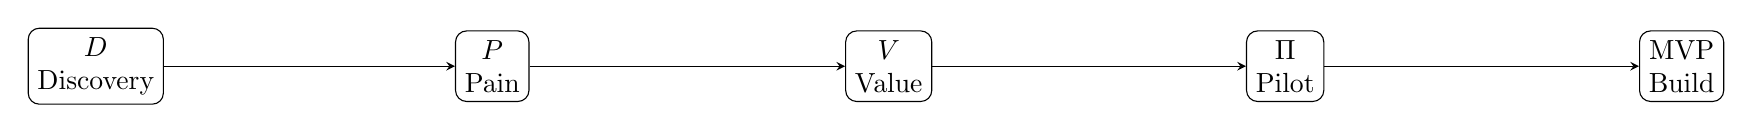
\begin{tikzpicture}[x=2.65cm,y=1.55cm,>=stealth]
\node[draw, rectangle, rounded corners, align=center] (d) at (0,0) {$D$\\Discovery};
\node[draw, rectangle, rounded corners, align=center] (p) at (1.9,0) {$P$\\Pain};
\node[draw, rectangle, rounded corners, align=center] (v) at (3.8,0) {$V$\\Value};
\node[draw, rectangle, rounded corners, align=center] (pi) at (5.7,0) {$\Pi$\\Pilot};
\node[draw, rectangle, rounded corners, align=center] (mvp) at (7.6,0) {$\mathrm{MVP}$\\Build};
\draw[->] (d) -- (p);
\draw[->] (p) -- (v);
\draw[->] (v) -- (pi);
\draw[->] (pi) -- (mvp);
\end{tikzpicture}
\caption{Transcript-derived reconstruction of the lecture's pre-build validation sequence.}
\end{figure}

This is the first place where the lecture sounds almost like a theorem. Not because it offers abstraction for its own sake, but because it insists on order. Entrepreneurship begins, in this telling, as disciplined listening. We do not yet know the business until we know how the customer names the problem.

\section{When Does the Idea Deserve More Investment?}

\subsection{Question \& Answer}

The next question is the natural one. Suppose we have an idea, perhaps a team, perhaps the beginning of some expenditure. When do we know that the idea is good enough to keep investing in?

John's answer is again subtractive. A problem may be very real and still fail to support a business. Magnitude of pain is not the same as business quality. What matters is whether one can actually get customers and then scale that process.

Let
\[
G = \text{``the idea is good enough to merit continued investment''},
\]
\[
A_{\mathrm{cust}} = \text{a workable customer-acquisition path},\qquad
S = \text{a path to scale}.
\]
Then the lecture's criterion may be summarized as
\begin{equation}
G \Leftarrow A_{\mathrm{cust}} \land S.
\end{equation}
At the same time, we must record the companion caution:
\begin{equation}
G \text{ is not certified by problem importance alone.}
\end{equation}

\begin{remark}
These formulas are deliberately modest. The lecture does not provide necessary-and-sufficient conditions; it provides a corrective emphasis. The point is that scale enters as a decisive filter, and that a substantial problem can still fall short of business viability.
\end{remark}

This is the chapter's conceptual hinge. We move from admiring the problem to interrogating the mechanism. A business becomes legible when it can travel from isolated value to repeatable customer capture.

\section{Perfectionism, Exposure, and the Use of Feedback}

\subsection{Question \& Answer}

Once the lecture has shifted us to customer acquisition and scale, the next obstacle appears almost automatically: perfectionism. What do we do when the founder keeps refining the product and never sends it out into the market?

John's answer is psychologically hard and operationally useful. Perfectionism is treated not as heroic standards but as insecurity. We are afraid to let anyone tell us that the baby is ugly, so we keep the baby hidden. The cost of that concealment is that the feedback loop never closes.

A transcript-faithful schematic is
\begin{equation}
\text{Prototype}_{0}
\xrightarrow{\text{feedback}}
\text{Prototype}_{1}
\xrightarrow{\text{feedback}}
\text{Prototype}_{2}
\rightarrow \cdots
\end{equation}
The lecture's actual language is more personal than this notation, but the structure is exact. We show something imperfect. We let the client react. We ask how to make it better for them. We then reshape the next version with more knowledge than we had before.

In the lecture's logic, the correction proceeds in five steps.
\begin{enumerate}
\item Recognize perfectionism as a refusal to risk judgment.
\item Present a differentiated but incomplete product anyway.
\item Let the client buy into shaping the fit.
\item Use the response to course-correct.
\item Replace concealment with an iterative learning loop.
\end{enumerate}

The important transition is that the customer is no longer merely a buyer at the far end of the process. The customer becomes part of the process by which the product finds its form.

\section{Failure First, Then Capital}

The lecture does something wise before answering the capital question. It pauses over failure. Adversity and setbacks, John says, are part of the journey itself. The destination may be an exit or an IPO, but the entrepreneur is formed by the obstacles encountered on the way there. This matters structurally because it repairs the founder's posture before it introduces the financial test.

Only then do we reach fundraising. John's answer again strips away fantasy. There is no magic number at which one suddenly becomes worthy of investment. Instead, there is a cluster of signs that make the business legible to outsiders. Let
\[
R_{\mathrm{raise}} = \text{fundraising readiness},\quad
U = \text{visible upside or potential},
\]
\[
A_{\mathrm{rep}} = \text{repeatable customer acquisition},\quad
\mathcal{P} = \text{a credible operating plan}.
\]
Then the lecture's logic may be compressed into
\begin{equation}
R_{\mathrm{raise}} \Leftarrow U \land A_{\mathrm{rep}} \land \mathcal{P} \land (\Delta \mathrm{MRR} > 0).
\end{equation}
Here \(\mathrm{MRR}\) denotes monthly recurring revenue, and the positive increment should be read cautiously: not as a hard threshold, but as a preferred sign that the business is moving in the right direction.

The lecture's derivation is clear enough to write out.
\begin{enumerate}
\item Use the modern environment to build and test cheaply.
\item If early revenue appears, recycle it back into the business.
\item Build broader traction rather than jumping prematurely to outside capital.
\item Show \(U\): there is room here for growth.
\item Show \(A_{\mathrm{rep}}\): customer acquisition is not a one-off miracle.
\item Show \(\mathcal{P}\): there is a plan, not merely a hope.
\item Prefer visible month-to-month improvement in revenue and \(\mathrm{MRR}\).
\item Only then take the business out for investment.
\end{enumerate}

\paragraph{Worked example.}
To keep the arithmetic concrete, suppose a company's recurring revenue moves from
\begin{align}
\mathrm{MRR}_0 &= \$8{,}000, &
\mathrm{MRR}_1 &= \$10{,}500.
\end{align}
Then
\begin{equation}
\Delta \mathrm{MRR} = \mathrm{MRR}_1 - \mathrm{MRR}_0 = \$2{,}500 > 0.
\end{equation}
This by itself proves nothing decisive. The lecture explicitly rejects a single magic threshold. But it does illustrate the kind of signal John wants to see: traction that is cumulative, directional, and increasingly repeatable.

The sequence matters. We do not raise money because the idea feels important. We raise money because the company is beginning to display a pattern.

\section{Scaling Rules, Marketing Channels, and Exit Discipline}

From here the lecture moves into later-stage operating judgment, but the sequence remains intelligible if we keep following the questions as they arise.

The first scaling rule concerns delegation. John's heuristic is crisp:
\begin{equation}
\text{Outsource if } c_{\mathrm{task}} < r_{\mathrm{founder}},
\end{equation}
where \(c_{\mathrm{task}}\) is the outside cost of a task and \(r_{\mathrm{founder}}\) is the founder's effective hourly value. If the role must become permanent, then the decision changes character: it becomes something to forecast and budget, not a casual productivity trick.

\paragraph{Worked example.}
Take the stylized numbers
\begin{align}
r_{\mathrm{founder}} &= \$200/\text{hr}, &
c_{\mathrm{task}} &= \$45/\text{hr}.
\end{align}
Then
\begin{equation}
c_{\mathrm{task}} < r_{\mathrm{founder}}
\qquad \Longrightarrow \qquad
\text{delegation is economically favored.}
\end{equation}
Again, this is not a complete decision rule. It omits quality variation, supervision cost, and strategic sensitivity. But the lecture presents it in precisely this spirit: as a practical scaling heuristic.

The next question concerns marketing, and here the lecture separates enterprise from consumer plays by channel mix rather than by ideology. In compact notation,
\begin{align}
M(\text{enterprise}) &= \{\text{email},\ \text{direct outreach},\ \text{cold calling (sometimes)},\ \text{social mix}\},\\
M(\text{consumer}) &\approx \{\text{social-heavy acquisition}\}.
\end{align}
The lecture does not argue that these sets are exhaustive. It argues that the route to the buyer depends on the buyer, and that founders must not confuse the channel logic of one market with that of another.

The exit question is then answered in deliberately plain terms. The best way to make the company sellable is to keep focusing on the bottom line and to keep moving the business forward efficiently. Institutional investors and potential acquirers notice sustained performance. In the chapter's shorthand,
\begin{equation}
E_{\mathrm{exit}} \uparrow
\qquad \text{as} \qquad
\mathrm{Revenue} \uparrow \ \text{and operating efficiency improves}.
\end{equation}
This is not a valuation model. It is a statement of posture. One does not optimize first for the story of selling; one optimizes first for performance that becomes difficult to ignore.

The mentor discussion follows naturally. The lecture rejects the fantasy that one great advisor can solve everything. One may need a coach for motivation, a mentor for sales, others for operations, and still others for more specialized matters. This fits the chapter's broader logic: entrepreneurship is too nuanced to be carried by a single source of certainty.

\section{Haymaker as the Applied Example}

Only after all of this does the lecture return in earnest to Haymaker, and that is exactly the right order. By now we have enough structure to see why the example matters.

Haymaker is described as a marketplace for temporary office and meeting spaces. Luxury homes, flex spaces, studios, and traditional commercial real estate are made available by the hour or by the day. The lecture's interest is not only in the inventory but in the pivot. A pre-pandemic idea aimed more broadly at coworking is re-read once work patterns change. Companies reduce their permanent real-estate footprints, distributed teams need periodic gathering places, and the product is redirected toward meeting spaces and flexible use.

We may compress that demand shift as
\begin{equation}
\text{distributed work}
\longrightarrow
\text{smaller permanent footprint}
\longrightarrow
\text{demand for flexible meeting and office inventory}.
\end{equation}
This is a fitting end for the chapter. We began with the abstract question of what it means to start and scale a company. We end with a concrete business whose current form is presented as the consequence of observing demand carefully and pivoting accordingly.

\section{Summary}

The lecture begins in public noise and ends in a fairly disciplined founder logic. First come teaser questions, fragments of advice, and the social fact of rejection. Then comes John Abraham's chronology: entry into tech sales, a launch in 2014, an exit in 2018, and a second company in motion. From there the argument sharpens.

We validate before we build. We interview decision-makers before we spend heavily. We ask what solving the problem would mean for the customer before we assume that the problem is worth building around. We do not call an idea good merely because the pain is real; we call it good when there is a path to customers and a path to scale. We resist perfectionism by exposing imperfect work to feedback. We read failure as formative. We treat capital as something earned by traction, repeatable acquisition, and a plan. We scale by delegating economically, market according to the buyer, prepare for exit by improving the bottom line, and rely on a circle of advisors rather than a single oracle.

What gives the interview its force is that it keeps replacing flattering descriptions with operational ones. The lecture does not ask us to admire entrepreneurship from a distance. It asks us to measure it by the sequence of tests through which a business becomes real.